\section{Moodle}
\subsection{Overview}
Modular Object-Oriented Dynamic Learning Environment, more commonly known as Moodle, is a learning management system founded in 2002 by Martin Dougiamas.
Supporting over 60\% of higher education institutions around the world, including UNSW, Moodle provides an open-source, personalised learning platform aimed at supporting both students and educators.
Moodle's modular design is centered around providing a personalised experience, giving users' the flexibility to build and access courses in a way that suits them.
With a vast library of plugins, and the ability for developers to design their own, Moodle really provides users with unlimited functionality.

\subsection{Dashboard}
When a logged-in user first accesses Moodle, they are directed to the Dashboard which consists of content blocks for each of the user's courses.
User's are provided with numerous ways to customise the dashboard, including:

\begin{itemize}
    \item Hiding and showing individual courses
    \item Filtering courses by past, present and future
    \item Sorting courses alphabetically or by date
    \item Displaying courses as cards or in a list
\end{itemize}

Users can use these customisation tools to organise the dashboard based on their needs and as a result, easily find a desired course.

\begin{figure}[h!]
    \centering
    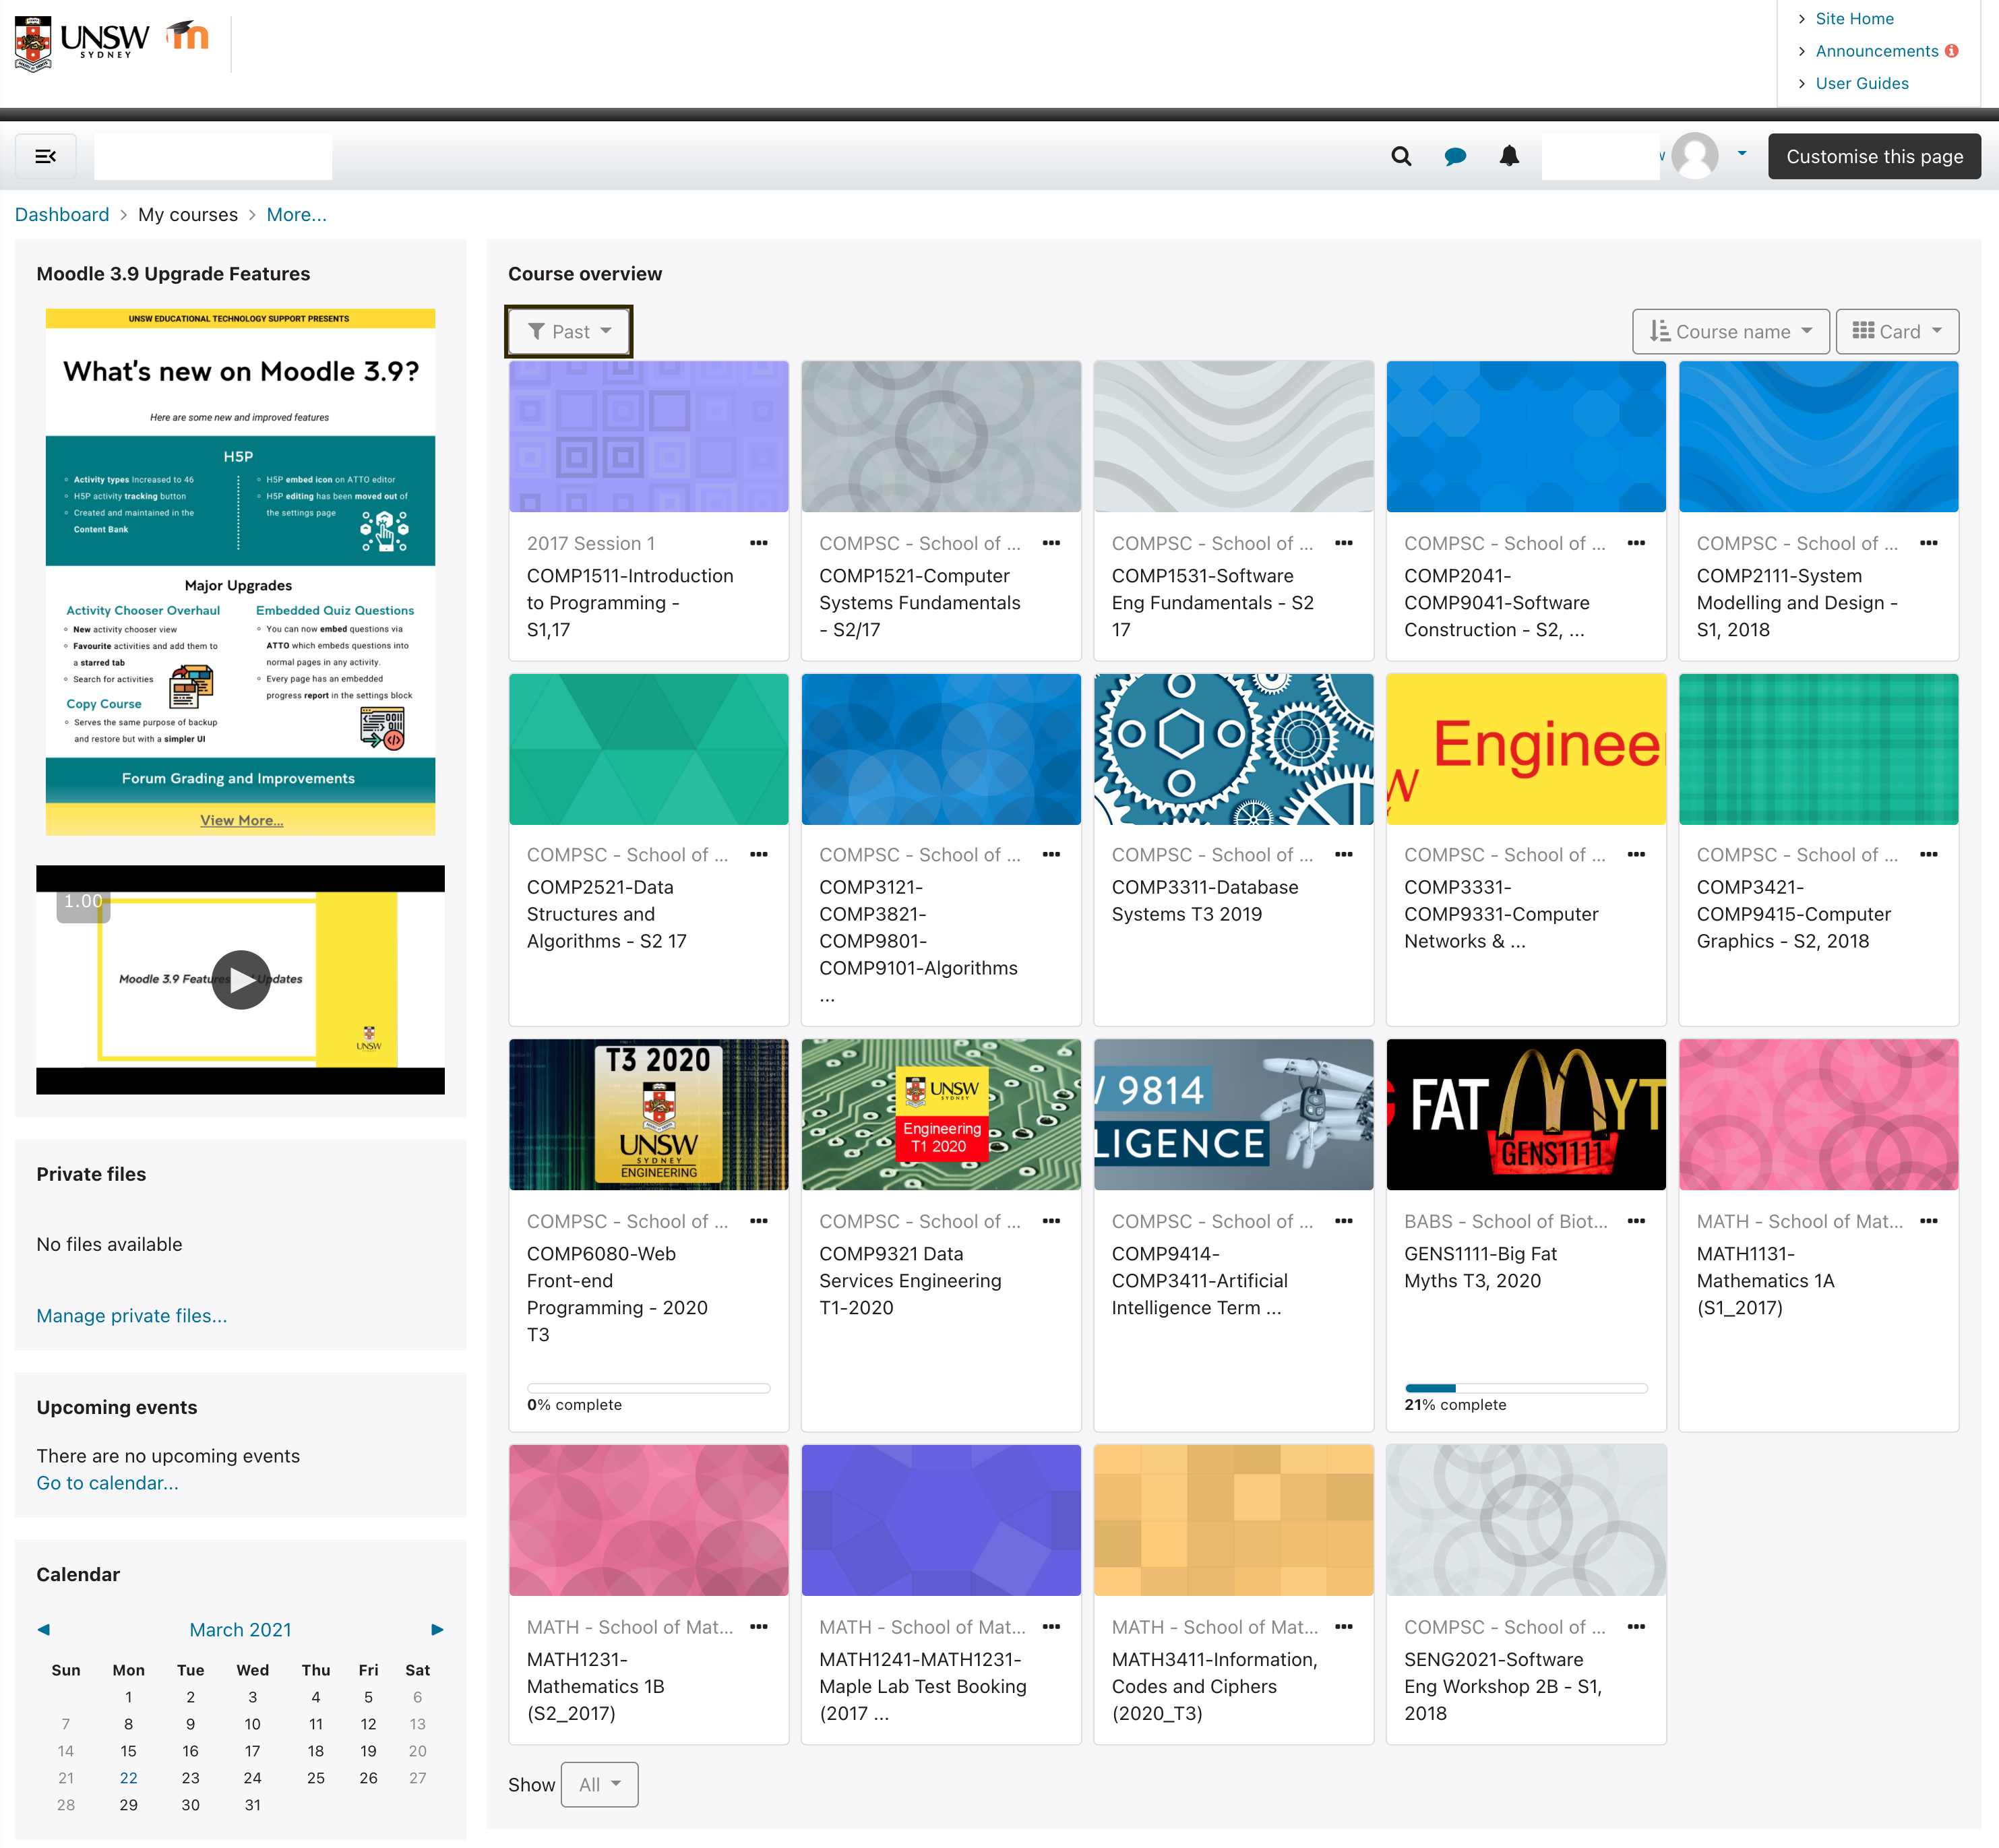
\includegraphics[scale=0.2]{moodle-dashboard}
    \caption{Moodle's Student Dashboard}
\end{figure}

\newpage

\subsection{Course Pages}
A course page consists of various links to resources. These links can be separated into collapsible subsections which help with the organisation of a course.
Course admins can customise the subsections based on how they would like to structure a course.
Course admins can also customise the way in which students work through course content by blocking access to resources until certain criteria have been met.

\begin{figure}[h!]
    \centering
    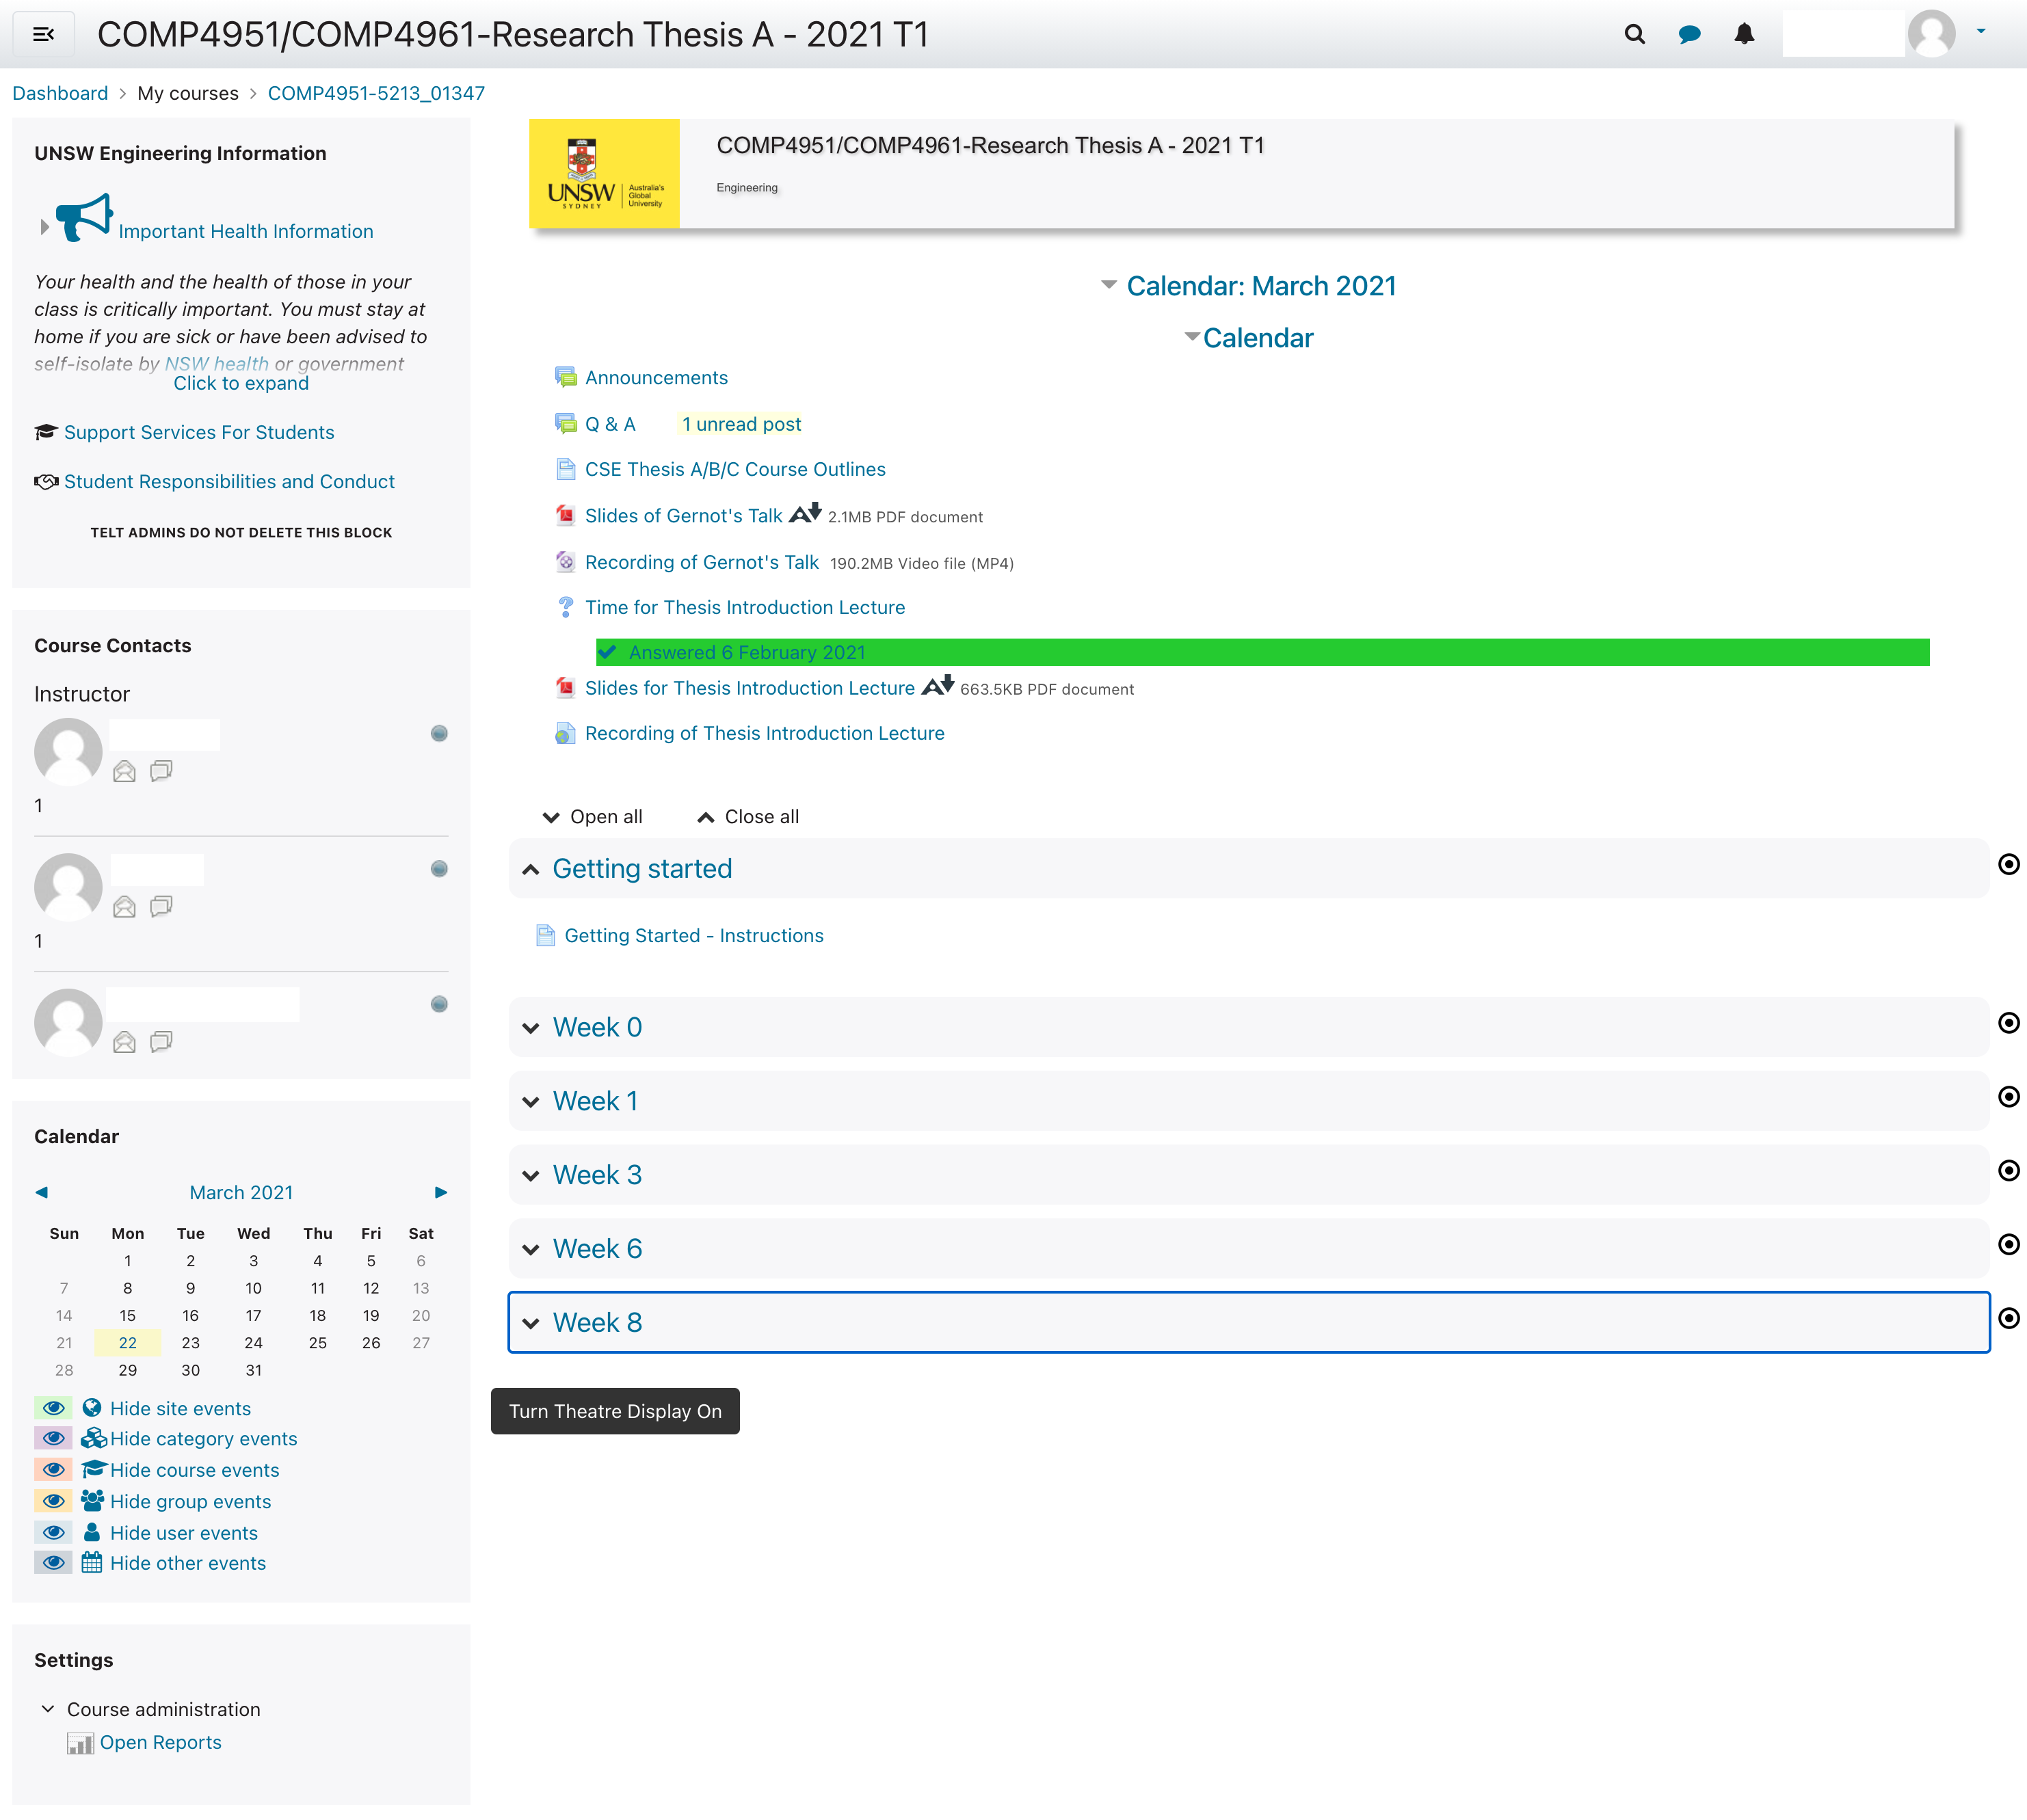
\includegraphics[scale=0.2]{moodle-course-page}
    \caption{Moodle's Student Course Page}
\end{figure}

The course page sidebar can also be edited to include different sections like course contacts, calendars, announcements and useful links.

Within a course page, students can access announcements, discussions, forums, quizzes, polls and course resources like lecture notes and assessment notifications.
Course admins can open assignment submissions and provide students with assessment feedback and grades.

\subsection{Forums}
Moodle provides course admins with the ability to create one or more forums attached to a course page.
Students and admins are able to post to the forum, reply to others, star posts and subscribe to conversations.
There is no easy way to search through forum posts which can make it difficult to find information, especially when the post list is long.
There is also no functionality for filtering sorting posts.
Overall, the forum functionality in Moodle is pretty basic and could use a lot of improvement when it comes to the organisation of information and the overall experience.

\begin{figure}[h!]
    \centering
    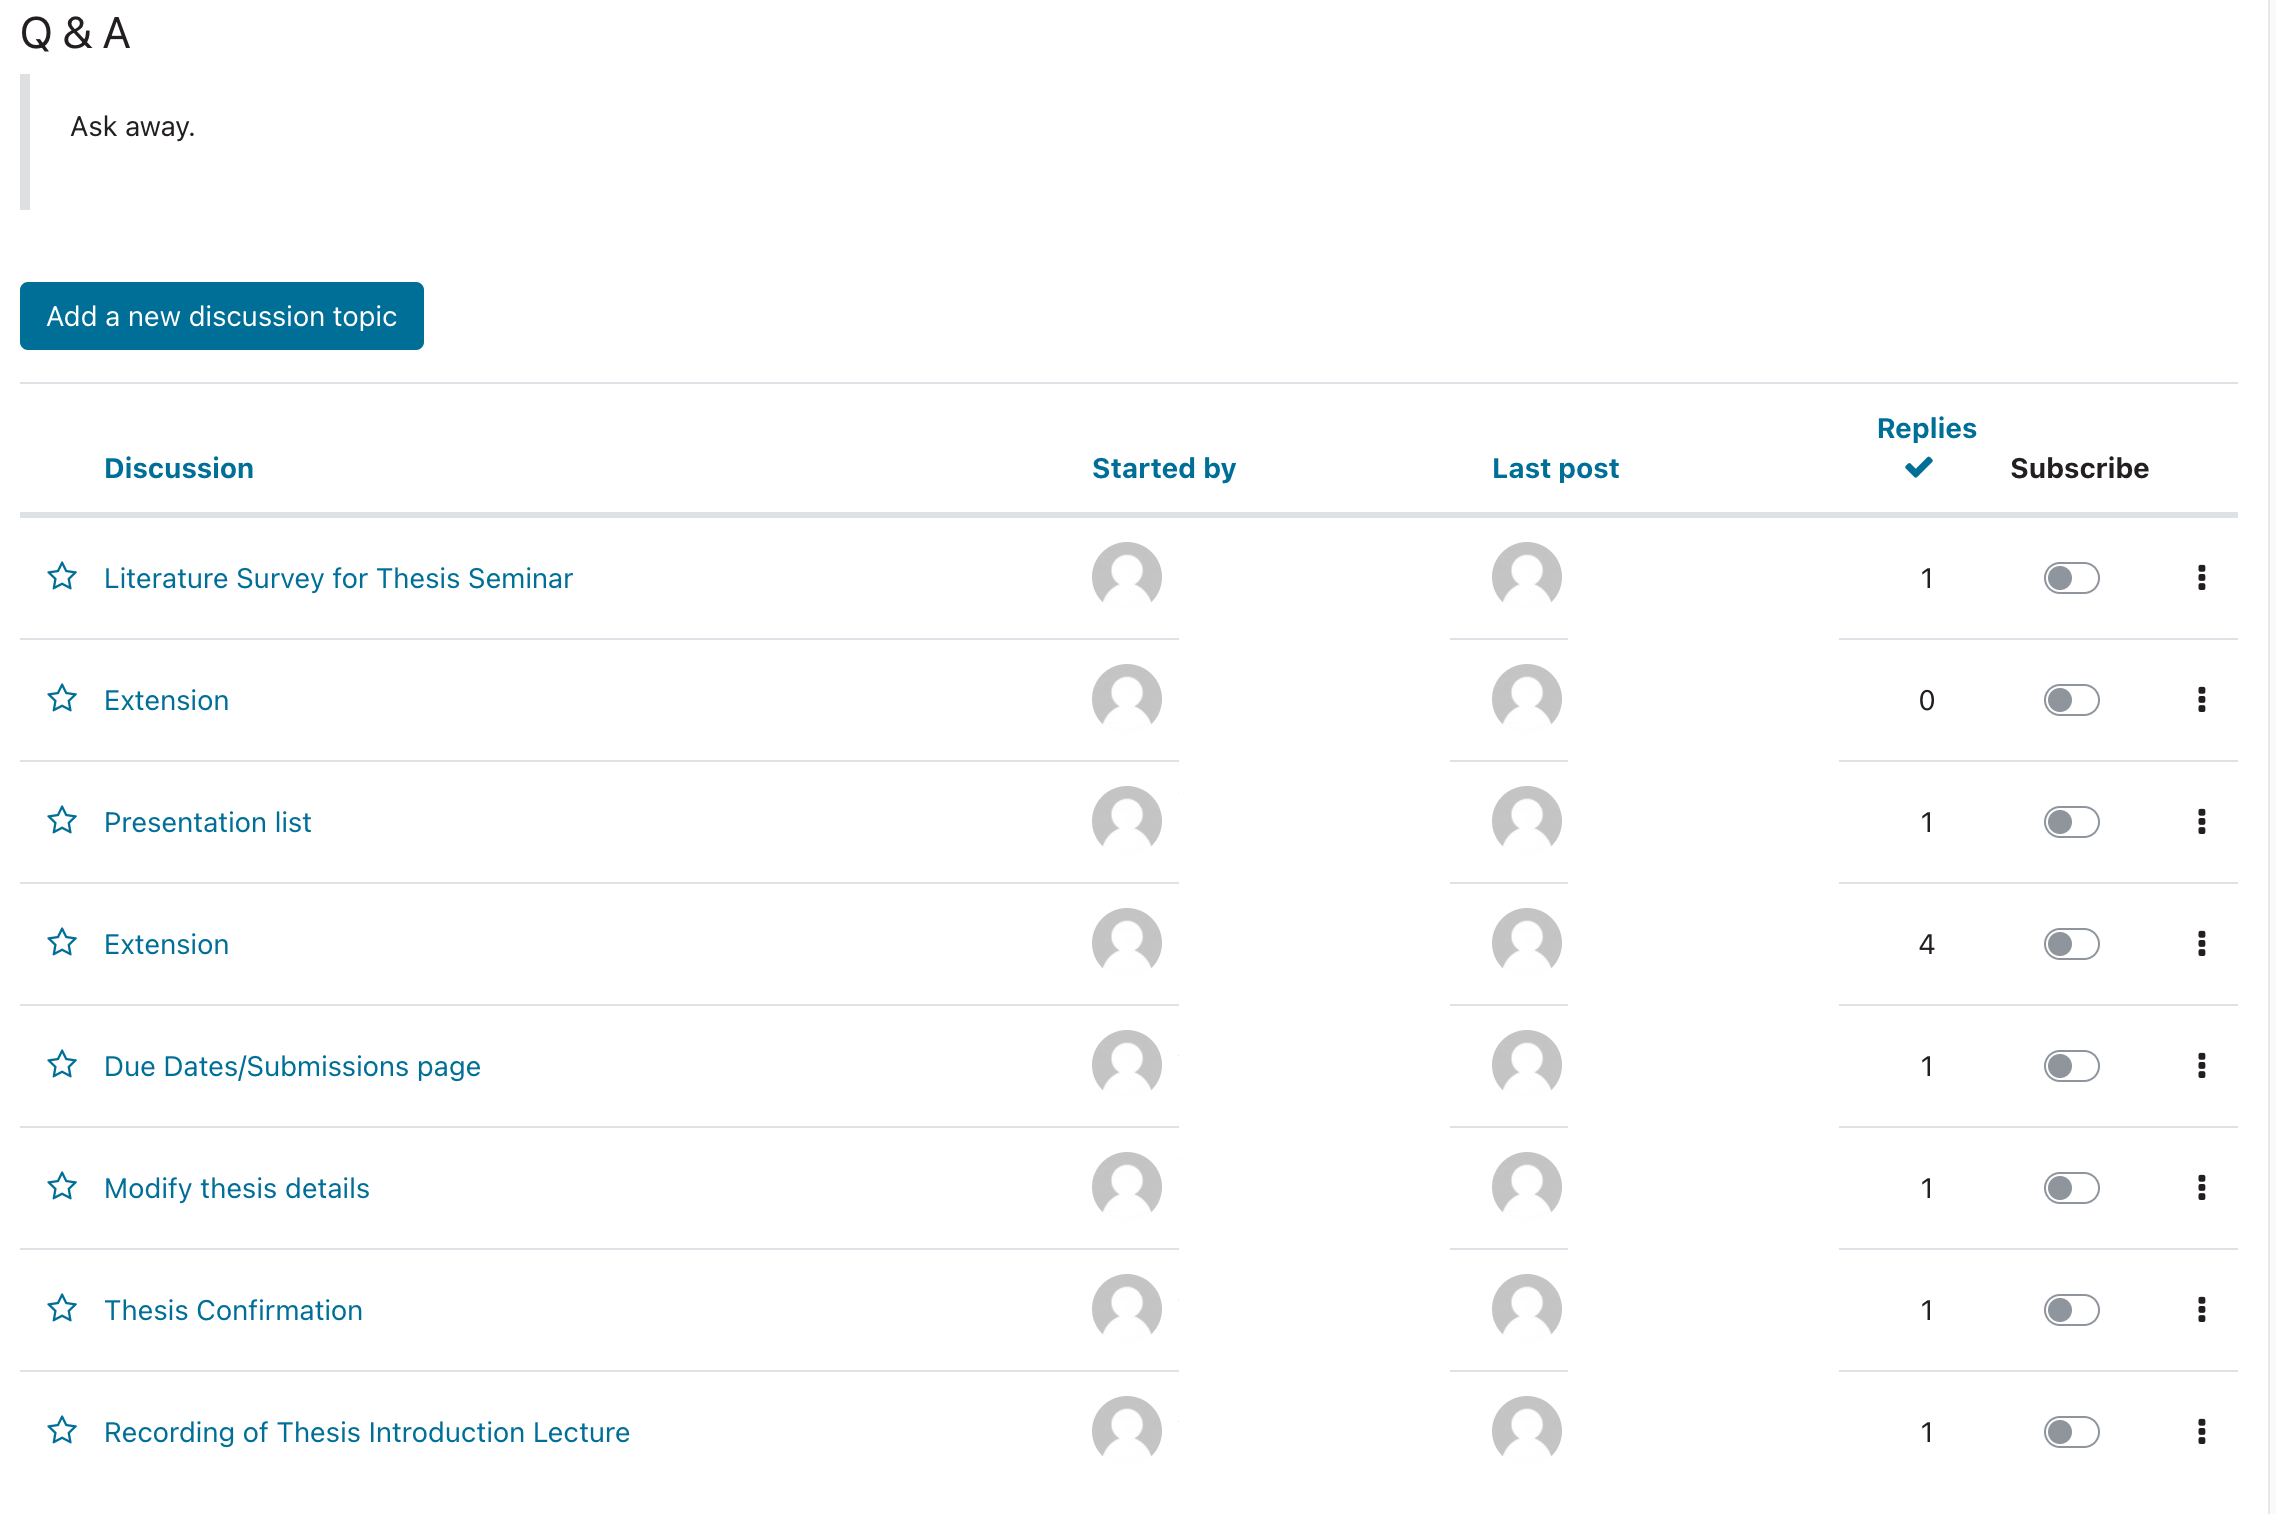
\includegraphics[scale=0.2]{moodle-forum}
    \caption{Moodle's Forums}
\end{figure}

\subsection{Performance and Accessibility}
The performance of Moodle is average, with Google's Lighthouse performance tool giving it a score between 60\% - 70\%, depending on the amount of content on the page.
A similar score was achieved for the accessibility of the website, with the biggest issues being lack of contrast between background and foreground colours, as well as HTML elements missing the appropriate attributes required for assistive technology.

\subsection{Data Migration}
Moodle provides users with the option to backup and restore data associated with a course.
Automated backups for courses can be set up to reduce the risk of losing data.
These backups can also be used to migrate data to a different platform.
Admins are able to easily select which parts of the course they would like to backup in the backup settings.
The backup files can then be easily saved and restored at any time.

\subsection{Conclusion}
While the user interface, performance and accessibility could use some improvements, Moodle successfully delivers all the required functionality need to support students and educators.